\documentclass{ctexart}

\usepackage{van-de-la-sehen}
\usepackage{van-le-trompe-loeil}

\usetikzlibrary{calc}

\def\equals{=}

\begin{document}

\section{常用半导体器件} % (fold)
\label{sec:常用半导体器件}

\subsection{半导体基础知识} % (fold)
\label{sub:半导体基础知识}

\subsubsection{本征半导体} % (fold)
\label{ssub:本征半导体}

纯净的具有晶体结构的半导体谓\emph{本征半导体}. 通常四价元素如\ce{Si}和\ce{Ge}的导电性介于半导体和绝缘体之间. 晶体中原子在空间形成排列整齐的点阵, 谓\emph{晶格}. 相邻原子之间存在共价键.
\par
常温下, 少数价电子由于热运动脱离共价键束缚变为自由电子, 同时在共价键中留下\emph{空穴}. 自由电子和空穴成对出现, 即二者数目相等. 外加电场时, 自由电子定向移动, 而价电子也将按一定方向填补空穴, 形成空穴电流. 两个效应运动方向相反, 电荷相反, 故电流为二者之和.
\par
运载电荷的粒子谓\emph{载流子}. 本征半导体的\emph{自由电子}和\emph{空穴}都是载流子.
\par
半导体在热激发下产生自由电子和空穴对的现象谓\emph{本征激发}. 自由电子运动过程中填补空穴谓\emph{复合}. 这一过程动态平衡, 故载流子浓度在一定温度下固定. 导电性能与温度正相关.
\[ n_i = p_i = K_1 T^{3/2} e^{-E\+_CO_/\pare{2kT}}. \]
其中$n_i$和$p_i$表示自由电子与空穴的浓度, $E\+_GO_$为热力学零度时破坏共价键所需能量, 即禁带宽度, $K_1$与半导体本身有关.

% subsubsection 本征半导体 (end)

\subsubsection{杂质半导体} % (fold)
\label{ssub:杂质半导体}

通过扩散工艺, 在本征半导体中掺入少量合适的杂质元素, 便可得到\emph{杂质半导体}.
\par
在纯净的硅晶体中掺入五价元素(如磷)可形成\emph{N型半导体}. 自由电子变为\emph{多数载流子}, 或\emph{多子}. 空穴变为\emph{少数载流子}, 或\emph{少子}. 杂质原子提供电子, 故谓\emph{施主原子}.
\par
在纯净的硅晶体中掺入三价元素(如硼)可形成\emph{P型半导体}. 自由电子变为{少子}. 空穴变为{多子}. 杂质原子提供空穴吸收电子, 故谓\emph{受主原子}.
\par
多子的浓度近似谓所掺杂杂质原子的浓度, 受温度影响小. 少子是本征激发形成的, 对温度较为敏感.

% subsubsection 杂质半导体 (end)

\subsubsection{PN结} % (fold)
\label{ssub:pn结}

将P型半导体与N型半导体制作在同一块硅片上, 交界面形成\emph{PN结}, 具有单向导电性. 空穴和电子的扩散导致P区出现负离子区而N区出现正离子区, 谓\emph{空间电荷区}, 或\emph{耗尽层}, 形成电场, 使载流子动态平衡.
\par
浓度差产生的运动, 谓\emph{扩散运动}. 电场力下载流子的运动, 谓\emph{漂移运动}.
\par
当外电压正极位于P端, 谓\emph{正向电压}. 此时P区空穴和N区自由电子被推向耗尽层, 耗尽层变窄, 原有平衡破坏, 扩散不断进行, PN结\emph{导通}.
\par
反之若正极位于N端, 则谓\emph{反向电压}. 此时空间电荷区变宽, 空间电荷区内电场增强, 更加阻止扩散, 而加剧漂移, 形成漂移电流, 由少子参与, 故电流极小. 总的$u$-$i$关系为
\[ i = I_S\pare{e^{\frac{qu}{kT}} - 1} = I_S\pare{e^{\frac{u}{U_T}}-1}, \quad U_T = \frac{kT}{q}. \]
其中$q$是电子电量. 常温下, $T\approx\SI{300}{\kelvin}$, $U_T\approx\SI{26}{\milli\volt}$.
\par
反向电压超过$U\+_(BR)_$后发生\emph{反向击穿}, 反向电流急剧增加. \emph{Zener击穿}谓耗尽层的大电厂破坏共价键, 发生于高掺杂. \emph{雪崩击穿}谓反向电压过大, 耗尽层电场使少子漂移速度加快, 撞出电子-空穴对, 新的电子指数重复这一过程.
\par
反向电压变化, 耗尽层电荷量亦变化. \emph{势垒电容}谓耗尽层变窄化所等效之电容$C_b$. PN结正向偏置时, P区扩散到N区的空穴和N区扩散到P区的自由电子谓\emph{非平衡少子}. \emph{扩散电容}谓电压变化时扩散去内非平衡少子的数目之变化之等效电容$C_d$. PN结的结电容为$C_j = C_b + C_d$, 这一值通常很小.

% subsubsection pn结 (end)

% subsection 半导体基础知识 (end)

\subsection{半导体二极管} % (fold)
\label{sub:半导体二极管}

\subsubsection{结构} % (fold)
\label{ssub:结构}

PN结用外壳封装, 加上电极引线形成半导体二极管.

% subsubsection 结构 (end)

\subsubsection{二极管的伏安特性} % (fold)
\label{ssub:二极管的伏安特性}

二极管只有当正向电压足够大时, 正向电流才从零端按指数上升. 这一电压谓开启电压$U\+_on_$.
\par
温度升高, 正向曲线左移, 反向曲线下移.

% subsubsection 二极管的伏安特性 (end)

\subsubsection{二极管的主要参数} % (fold)
\label{ssub:二极管的主要参数}

主要参数如左列:
\begin{cenum}
    \item 最大整流电流$I_F$, 即二极管长期运行时允许通过的最大平均电流;
    \item 最高反向工作电压$U_R$, 通常为击穿电压$U\+_(BR)_$的一半;
    \item 反向电流$I_R$, 即未被击穿时的反向电流;
    \item 最高工作频率$f_M$, 超过此频率结电容可能导致二极管不能呈现良好的单向导电性.
\end{cenum}

% subsubsection 二极管的主要参数 (end)

\subsubsection{二极管的等效电路} % (fold)
\label{ssub:二极管的等效电路}

\begin{figure}[ht]
    \centering
    \begin{subfigure}{3.5cm}
        \centering
        \begin{tikzpicture}[domain=0:1]
            \draw[->] (-1.5,0) -- (1.5,0) node[below] {$u$};
            \draw[->] (0,0) node[below left] {$O$} -- (0,3) node[left] {$i$};
            \draw[dashed] plot[id=exp] function{0.3*exp(x*2.3)-0.3} node[right] {};
            \draw[ultra thick] (-1.2,0) -- (0,0) -- (0, 2.8);
            \draw (-1.5,-2) to[Do] (1.5,-2);
            \draw[color=white] (-1.5,-3) (1.5,-3);
        \end{tikzpicture}
        \caption{理想二极管}
    \end{subfigure}
    \begin{subfigure}{3.5cm}
        \centering
        \begin{tikzpicture}[domain=0:1]
            \draw[->] (-1.5,0) -- (1.5,0) node[below] {$u$};
            \draw[->] (0,0) node[below left] {$O$} -- (0,3) node[left] {$i$};
            \draw[dashed] plot[id=exp] function{0.3*exp(x*2.3)-0.3} node[right] {};
            \draw[ultra thick] (-1.2,0) -- (1,0) node[below] {$U\+_on_$} -- (1, 2.8);
            \draw (-1.5,-2) to[Do] (0,-2) to[battery1,l=$U\+_on_$] (1.5,-2);
            \draw[color=white] (-1.5,-3) (1.5,-3);
        \end{tikzpicture}
        \caption{正向时$u$为常量}
        \label{fig:正向时u为常量}
    \end{subfigure}
    \begin{subfigure}{3.5cm}
        \centering
        \begin{tikzpicture}[domain=0:1]
            \draw[->] (-1.5,0) -- (1.5,0) node[below] {$u$};
            \draw[->] (0,0) node[below left] {$O$} -- (0,3) node[left] {$i$};
            \draw[dashed] plot[id=exp] function{0.3*exp(x*2.3)-0.3} node[right] {};
            \draw[ultra thick] (-1.2,0) -- (0.434268,0) node[below] {$U\+_on_$} -- (1, 2.45788);
            \draw[dashed] (0,1.58896) -- (0.8,1.58896) -- (0.8,0);
            \draw (-1.5,-2) to[Do] (-0.5,-2) to[battery1,l=$U\+_on_$] (0.5,-2) to[resistor,R=$r_D$] (1.5,-2);
            \draw[color=white] (-1.5,-3) (1.5,-3);
        \end{tikzpicture}
        \caption{正向时$i\propto \pare{u-U\+_on_}$}
        \label{fig:正向时线性}
    \end{subfigure}
    \caption{伏安特性折线化得到的等效电路}
\end{figure}

\begin{sample}
    \begin{ex}
        二极管为硅管, 电阻$R=\SI{10}{\kilo\volt}$, 分析电压源分别为$\SI{30}{\volt}$, $\SI{6}{\volt}$和$\SI{1.5}{\volt}$时的回路电流.
    \end{ex}
    \centerline{\begin{tikzpicture}
        \draw (0,0) to[battery1,invert,l=$V$] (0,2) to [Do,v=$U_D$,i=$I$] (3,2) to [resistor,v=$U_R$,R=$R$] (3,0) -- (0,0);
    \end{tikzpicture}}
    \begin{solution}
        对于硅管, 导通电压为$\SI{0.6}{\volt}\sim \SI{0.8}{\volt}$.
        \begin{cenum}
            \item 当$V=\SI{30}{\volt}$, $V$是$U_D$的几十倍, 可认为$R$上电压近似为电源电压, $I\approx V/R = \SI{3}{\milli\ampere}$.
            \item 当$V=\SI{6}{\volt}$, 电源电压是$U_D$的几倍, 可认为二极管服从\cref{fig:正向时u为常量}中的特性曲线. 取$U_D = U\+_on_ = \SI{0.7}{\volt}$, 回路电流
            \[ I \approx \frac{V - U\+_on_}{R} = \SI{0.53}{\milli\ampere}. \]
            \item 当$V=\SI{1.5}{\volt}$, 接近于$U_D$, 需要采用\cref{fig:正向时线性}中的特性曲线. 设$U\+_on_ = \SI{0.55}{\volt}$, $r_D = \SI{200}{\ohm}$, 则
            \[ I = \frac{V - U\+_on_}{r_D+R} = \frac{\pare{1.5-0.55}\SI{}{\volt}}{\pare{0.2+10}\SI{}{\kilo\ohm}} \approx \SI{93}{\micro\ampere}. \qedhere \]
        \end{cenum}
    \end{solution}
\end{sample}

\begin{sample}
    \begin{ex}
        设二极管导通电压$U_D \approx \SI{0.7}{\volt}$, 估算开关断开和闭合时的输出电压数值.
    \end{ex}
    \centerline{\begin{tikzpicture}
        \draw (0,0) to[battery1, invert,l=$\stackrel{\displaystyle V_1}{\scriptstyle \pare{\SI{6}{\volt}}}$] (0,3) to[Do,l=$D$,-*] (1.8,3) -- (3,3) to[resistor,R=$R$,v=$U_O$] (3,0) to[short,-*] (1.8,0) -- (0,0);
        \draw (1.8,0) to[battery1, invert,l=$\stackrel{\displaystyle V_2}{\scriptstyle \pare{\SI{12}{\volt}}}$] (1.8,1.5) to[nos,l=$S$] (1.8,3);
    \end{tikzpicture}}
    \begin{solution}
        开关断开时, 二极管正向导通, 输出电压
        \[ U_O = V_1 - U_D = \pare{6-0.7}\SI{}{\volt} = \SI{5.3}{\volt}. \]
        闭合时二极管截止,
        \[ U_O = V_2 = \SI{12}{\volt}. \]
    \end{solution}
\end{sample}
通过在二极管的$u$-$i$特性曲线中以切线近似, 可以得到二极管的微变等效电路, 其中
\[ \rec{r_d} \approx \+d{u_D}d{i_D} = \+dud{\brac{I_S\pare{e^{u/U_T} - 1}}} \approx \frac{I_S}{U_T}e^{u/U_T} \approx \frac{I_D}{U_T},\quad r_d\approx \frac{U_T}{I_D}. \]

% subsubsection 二极管的等效电路 (end)

\subsubsection{稳压二极管} % (fold)
\label{ssub:稳压二极管}

\begin{figure}[ht]
    \centering
    \begin{subfigure}[b]{4cm}
        \centering
        \begin{tikzpicture}
            \draw (0,0) to [zDo,invert,l=$D_Z$] (3,0);
        \end{tikzpicture}
        \caption{稳压二极管符号}
    \end{subfigure}
    \begin{subfigure}[b]{4cm}
        \centering
        \begin{tikzpicture}
            \draw (0,0) to[short,-*] (0.5,0) -- (0.5,2) to[Do,invert,l=$D_1$] (3.5,2) to[short,-*] (3.5,0) -- (4,0);
            \draw (0.5,0) to[Do,l=$D_2$] (1.5,0) to[battery,l=$U_Z$] (2.5,0) to[resistor,R=$r_d$] (3.5,0);
        \end{tikzpicture}
        \caption{稳压二极管等效}
    \end{subfigure}
    \caption{稳压二极管符号与等效}
\end{figure}
稳压二极管正向特性为指数曲线, 反向电压大到一定程度($U_Z$)则发生击穿, 此时曲线及其陡峭, 只要反向控制电流不超过某阈值就不会因过热而损坏. 主要参数有
\begin{cenum}
    \item 稳定电压$U_Z$, 即在规定电流下稳压管的反向击穿电压.
    \item 稳定电流$I_Z$或$I\+_Zmin_$, 即稳压管工作在稳压状态时的参考电流, 电流低于次值无法稳压.
    \item 额定功耗$P\+_ZM_$, 即$U_ZI\+_ZM_$, 其中$I\+_ZM_$为最大稳定电流, 超过此值可能损坏二极管.
    \item 动态电阻$r_z$, 即工作在稳压区时的$\Delta U_Z/\Delta I_Z$, 越高稳压性能越好.
    \item 温度系数$\alpha$, 即$\Delta U_Z/\Delta T$. $U_Z<\SI{4}{\volt}$属于Zener击穿, 具有负温度系数. $U_Z>\SI{7}{\volt}$属于雪崩击穿, 具有正温度系数. 在二者之间$\alpha \approx 0$.
\end{cenum}
为了保证恰当的工作电流, 需要在稳压电路中串联一个电阻以限制电流.
\begin{sample}
    \begin{ex}
        若稳压管$U_Z = \SI{6}{\volt}$, $I\+_Zmin_ = \SI{5}{\milli\ampere}$, $I\+_Zmax_ = \SI{25}{\milli\ampere}$, 负载电阻$R_L = \SI{600}{\ohm}$, 求限流电阻$R$的取值范围.
    \end{ex}
    \centerline{\begin{tikzpicture}
        \draw (0,3) to[resistor,R=$R$, i=$I_R$,o-*] (3,3) to [zDo,invert,l_=$D_Z$,i_=$I_{D_Z}$, -*] (3,0) to[short, -o] (0,0) (0,3) to[open,v=$U_1\equals\SI{10}{\volt}$] (0,0) (3,3) to[short,-o] (4.5,3) to[resistor,R=$R_L$,v=$U_O$,i=$I_L$,-o] (4.5,0) -- (3,0);
    \end{tikzpicture}}
    \begin{solution}
        $I_L = U_Z/R_L = \SI{10}{\milli\ampere}$, $I_R = I_{DZ} + I_L = \pare{15\sim 35}\SI{}{\milli\ampere}$, $U_R = U_1 - U_Z = \SI{4}{\volt}$,
        \[ R = \frac{\SI{4}{\volt}}{\pare{15\sim 35}\SI{}{\milli\ampere}} = \pare{114\sim 267}\SI{}{\ohm}. \qedhere \]
    \end{solution}
\end{sample}

% subsubsection 稳压二极管 (end)

\subsubsection{其它类型二极管} % (fold)
\label{ssub:其它类型二极管}

\paragraph{发光二极管} % (fold)
\label{par:发光二极管}

发光二极管的符号为\tikz[baseline=0.0cm] \draw (0,0) to[leDo] (2,0);. 只有当正向电压足够大时才发光. 红色大约为$\SI{1.6}{\volt}\sim \SI{1.8}{\volt}$, 绿色大约为$\SI{2}{\volt}$.

% paragraph 发光二极管 (end)

\paragraph{光电二极管} % (fold)
\label{par:光电二极管}

光电二极管的符号为\tikz[baseline=0.0cm] \draw (0,0) to[pDo] (2,0);. 无光照时与普通二极管无异. 有光照时, 特性曲线下移, 可作为恒流源. 

% paragraph 光电二极管 (end)

\begin{sample}
    \begin{ex}
        已知发光二极管的导通电压$U_D = \SI{1.6}{\volt}$, 正向电流$\SI{5}{\milli\ampere}\sim\SI{20}{\milli\ampere}$才能发光, 问开关处于何种位置发光二极管才能发光, 以及发光时$R$的取值范围.
    \end{ex}
    \centerline{\begin{tikzpicture}
        \draw (0,0) to[battery1, invert, l=$\stackrel{\displaystyle V}{\scriptstyle\pare{\SI{6}{\volt}}}$] (0,3) to[resistor,R=$R$,-*] (1.8,3) to[nos,l=$S$, invert, -*] (1.8,0) -- (0,0) (1.8,3) -- (3,3) to[pDo,l=$D$] (3,0) -- (1.8,0);
    \end{tikzpicture}}
    \begin{solution}
        只有当开关断开时会发光. 此时
        \[ R = \frac{V-U_D}{I\+_Dmin_ \sim I\+_Dmax_} = \pare{\frac{6-1.6}{5\sim 20}}\SI{}{\kilo\ohm} = \pare{0.22\sim 0.88}\SI{}{\kilo\ohm}. \qedhere \]
    \end{solution}
\end{sample}

% subsubsection 其它类型二极管 (end)

% subsection 半导体二极管 (end)

\subsection{晶体三极管} % (fold)
\label{sub:晶体三极管}

\subsubsection{结构与类型} % (fold)
\label{ssub:结构与类型}

\begin{figure}[ht]
    \centering
    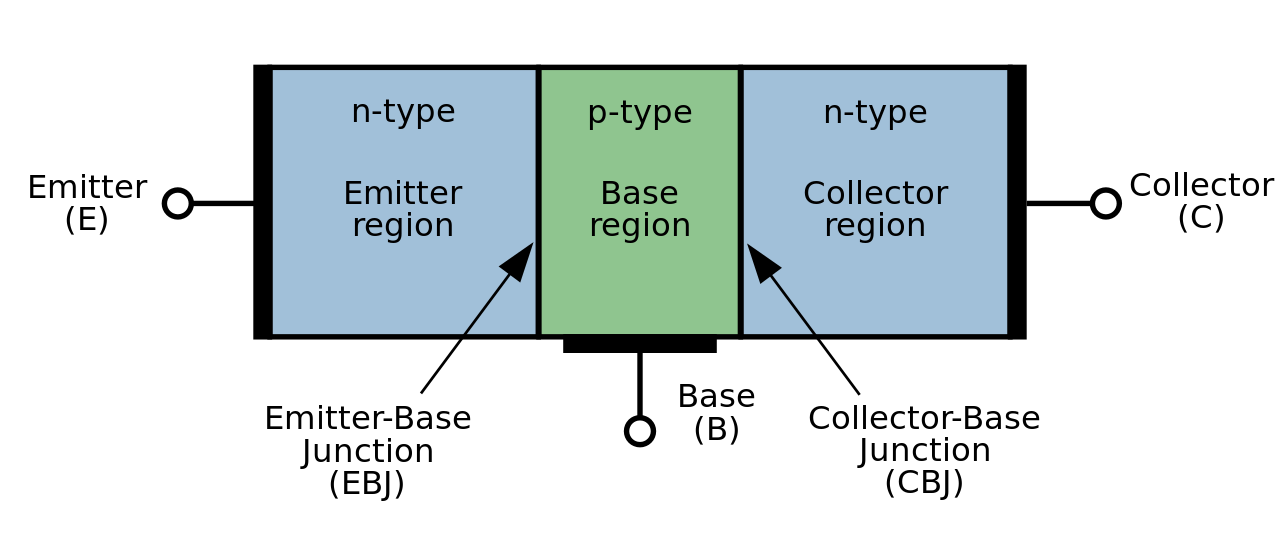
\includegraphics[width=10cm]{src/NPN_BJT.png}
    \caption{}
\end{figure}

晶体三极管中有两种不同载流子参与导电, 故谓双极型晶体管(BJT), 又谓半导体三极管, 简称晶体管. 根据不同掺杂方式在同一硅片上制造三个掺杂区域, 可形成
\begin{cenum}
    \item NPN型晶体管, 符号如\tikz[baseline=0.0cm] \draw (0,0) node[npn] {};.
    \item 或者PNP型晶体管, 符号如\tikz[baseline=0.0cm]\draw (0,0) node[pnp] {};.
\end{cenum}

% subsubsection 结构与类型 (end)

\subsubsection{共射放大电路} % (fold)
\label{ssub:共射放大电路}

\begin{figure}[ht]
    \centering
    \begin{tikzpicture}
        \draw (2,3.5) node[npn] (npn1) {};
        \draw (0,0) to[battery1,invert,l=$V\+_BB_$] (0,1) to[european voltage source,v<=$\Delta u_1$] (0,2) to[resistor,R=$R_b$] (0,3) |- (npn1.B);
        \draw (npn1.E) --++ (0,-3) node[circ] (circE) {};
        \draw (circE) --++(2,0) node[circ] (circVCCN) {};
        \draw (npn1.C) |- ++(2,0.5) node[circ] (circVCCP) {};
        \draw (0,0) |- (circE);
        \draw (circVCCP) to[resistor,R=$R_c$] ($(circVCCP) + (0,-2)$) to[battery,l=$V\+_CC_$] (circVCCN);
        \draw (circVCCP) to[short,-o] ($(circVCCP) + (1,0)$);
        \draw (circVCCN) to[short,-o] ($(circVCCN) + (1,0)$);
        \draw ($(circVCCP) + (1,0)$) to[open,v^=$u_O$] ($(circVCCN) + (1,0)$);
        \draw (circE) node[ground] {};
    \end{tikzpicture}
    \caption{基本共射放大电路}
    \label{fig:基本共射放大电路}
\end{figure}
$\Delta u_1$为输入信号, 接入基极-发射极回路, 谓输入回路. 放大后信号在集电极-发射极回路, 谓输出回路. 发射极是两个回路的公共端, 故谓\emph{共射放大电路}. 晶体管工作在放大状态的条件是\emph{发射结正向偏置且集电极反向偏置}. 因此应有$V\+_CC_ > V\+_BB_$.
\begin{table}
    \centering
    \begin{tabular}{cm{3cm}m{2cm}m{2cm}}
    \toprule
     & \+:c1{c}{基区(P)-发射区(N)} & \+:c1{c}{基区(P)-集电区(N)} & \+:c1{c}{进入基区(P)} \\
    \midrule
    空穴(P) & 空穴(P)扩散$I\+_EP_$ & 平衡少子漂移$I\+_CBO_$ \\
    \midrule
    电子(N) & 电子(N)扩散$I\+_EN_$ 复合$I\+_BN_$ & 未复合$I\+_CN_$ & \\
    \midrule
    总和 & $I\+_EP_\ll I\+_EN_$, $I\+_E_ = I\+_EP_ + I\+_EN_ = I\+_CN_ + I\+_BN_ + I\+_EP_$ & $I_C = I\+_CN_ + I\+_CBO_$ & $I_B = I\+_BN_ +$ $I\+_EP_ - I\+_CBO_$ $= I'_B - I\+_CBO_$ \\
    \midrule
    & \+:c3{c}{$I_E = I_B + I_C$} \\
    \bottomrule
    \end{tabular}
\end{table}
\par
共射直流电流放大系数谓
\[ \conj{\beta} = \frac{I\+_CN_}{I'\+_B_} = \frac{I_C - I\+_CBO_}{I_B+I\+_CBO_},\quad I_C = \conj{\beta}I_B + \underbrace{\pare{1+\conj{\beta}}I\+_CBO_}_{I\+_CEO_}. \]
$I\+_CBO_$是发射极开路时, 集电结的反向饱和电路. $I\+_CEO_$是穿透电流, 即基极开路时, 集电极与发射极之间的电流. 通常$I_B \gg I\+_CBO_$, $\conj{\beta}\gg 1$, 故
\[ I_C \approx \conj{\beta}I_B,\quad I_E \approx\pare{1+\conj{\beta}}I_B. \]
若有输入电压$\Delta u_1$的作用, 则相应的$I_B$和$I_C$会附加$\Delta i_B$和$\Delta i_C$, 而共射交流电流放大系数谓
\[ \beta = \frac{\Delta i_C}{\Delta i_B}. \]
在$\Delta i_B$不大的情形下, 可认为
\[ \beta \approx \conj{\beta}. \]
\par
以发射极电流作为输入电流, 集电极电流作为输出电流时, 共基直流电流放大系数谓
\[ \conj{\alpha} = \frac{I\+_CN_}{I_E},\quad I_C = \conj{\alpha} + I\+_CBO_. \]
由$I_E = I_C + I_B$, 可得
\[ \conj{\beta} = \frac{\conj{\alpha}}{1-\conj{\alpha}},\quad \conj{\alpha} = \frac{\conj{\beta}}{1+\conj{\beta}}. \]
类似定义
\[ \alpha = \frac{\Delta i_C}{\Delta i_E} = \frac{\beta}{1+\beta}. \]
通常$\beta \gg 1$, $\alpha \approx 1$, $\beta \approx \conj{\beta}$, $\alpha \approx \conj{\alpha}$.

% subsubsection 共射放大电路 (end)

\subsubsection{共射特性曲线} % (fold)
\label{ssub:共射特性曲线}

输入特性曲线谓$u\+_CE_$一定之条件下, 基极电流$i_B$与发射结压降$u\+_BE_$之间的关系.
\begin{figure}[htb]
    \centering
    \begin{tikzpicture}
        \draw[->] (0,0) -- (4,0) node[below] {$u\+_BE_$};
        \draw[->] (0,0) node[below left] {$O$} -- (0,4) node[left] {$i_B$};
        \draw[domain=0:1.1] plot[id=exp] function{0.3*exp(x*2.3)-0.3} node[left] {$u\+_CE_=0$};
        \draw[domain=0:1.95] plot[id=exp2] function{0.3*exp(x*1.3)-0.3} node[above] {$\SI{0.5}{\volt}$};
        \draw[domain=0:2.5] plot[id=exp3] function{0.3*exp(x*1)-0.3} node[right] {$\ge\SI{1}{\volt}$};
    \end{tikzpicture}
    \caption{输入特性曲线}
\end{figure}
$u\+_CE_$增大, 曲线右移, 因为在基区参与复合的非平衡少子随$u\+_CE_$的增大而减小.
\par
输出特性曲线谓$i_B$一定之条件下, 集电极电流$i_C$与管压降$u\+_CE_$之间的关系.
\begin{figure}[htb]
    \centering
    \begin{tikzpicture}
        \draw[->] (0,0) -- (4,0) node[below] {$u\+_CE_$};
        \draw[->] (0,0) node[below left] {$O$} -- (0,4) node[left] {$i_C$};
        \draw[domain=0:4] plot[id=atan] function{0.7*0.1*atan(x/0.1*60)} node[right] {$i_B=0$};
        \draw[domain=0:4] plot[id=atan] function{0.7*atan(x*60)} node[right] {$i_{B1}$};
        \draw[domain=0:4] plot[id=atan] function{0.7*2*atan(x/2*60)} node[right] {$i_{B2}$};
        \draw[domain=0:4] plot[id=atan] function{0.7*3*atan(x/3*60)} node[right] {$i_{B3}$};
        \draw[domain=0:4] plot[id=atan] function{0.7*4*atan(x/4*60)} node[right] {$i_{B4}$};
        \draw[domain=0:0.65,dashed] plot[] function{5*exp(x)-5} node {};
        \draw[dashed] (-0.3,2.2) -- (2,2.2) (-0.3,3.3) -- (2,3.3);
        \draw (-0.3,2.75) node[left] {$\Delta i_C$};
        \draw (0.3,3.5) -- (2,4.5) node[right] {饱和区} (2,2.65) node[right] {放大区} (2,0.05) -- (1,-0.2) node[below] {截止区};
    \end{tikzpicture}
    \caption{输出特性曲线}
    \label{fig:晶体三极管输出特性曲线}
\end{figure}
晶体管有三个工作区域:
\begin{cenum}
    \item 截止区: 发射结小于开启电压, 集电结反向偏置, $u\+_BE_ \le U\+_on_$且$u\+_CE_ > u\+_BE_$, 此时$I_B = 0$.
    \item 放大区: 发射结正向偏置, 集电结反向偏置, $u\+_BE_ > U\+_on_$且$u\+_CE_ \ge u\+_BE_$, 此时$I_C = \conj{\beta}I_B$, $\Delta i_C = \beta \Delta i_B$.
    \item 饱和区: 发射结与集电结都处于正向偏置, $u\+_BE_ > U\+_on_$且$u\+_CE_ < u\+_BE_$, 此时$I_C$与$I_B$相关.
\end{cenum}

% subsubsection 共射特性曲线 (end)

\subsubsection{主要参数} % (fold)
\label{ssub:主要参数}

$\conj{\beta}$, $\conj{\alpha}$, $\beta$, $\alpha$, $I\+_CBO_$, $I\+_CEO_$如前所述. 考虑到结电容的存在, 当频率上升时共射电流放大系数下降, 下降到$1$时的信号频率谓特征频率$f_T$.
\par
此外还有最大集电极耗散功率$P\+_CM_$, 最大集电极电流$I\+_CM_$, 极间反向击穿电压等.

% subsubsection 主要参数 (end)

\subsubsection{温度影响} % (fold)
\label{ssub:温度影响}

温度上升, $I\+_CBO_$和$I\+_CEO_$上升, 输入特性曲线左移, 输出特性曲线上移.

% subsubsection 温度影响 (end)

\begin{sample}
    \begin{ex}
        设有若干NPN晶体管的电位如下表, b-e间开启电压为$\SI{0.5}{\volt}$, 则相应的工作状态可推断如下.
    \end{ex}
    \centerline{
    \begin{tabular}{ccccc}
        \toprule
        晶体管 & $T_1$ & $T_2$ & $T_3$ & $T_4$ \\
        \midrule
        基极直流电位$U_B/\SI{}{\volt}$ & $0.7$ & $1$ & $-1$ & $0$ \\
        \midrule
        发射极直流电位$U_E/\SI{}{\volt}$ & $0$ & $0.3$ & $-1.7$ & $0$ \\
        \midrule
        集电极直流电位$U_C/\SI{}{\volt}$ & $5$ & $0.7$ & $0$ & $15$ \\
        \midrule
        工作状态 & 放大 & 饱和 & 放大 & 截止 \\
        \bottomrule
    \end{tabular}
    }
\end{sample}
\begin{sample}
    \begin{ex}
        在一个单管放大电路中, 电源电压为$\SI{30}{\volt}$, 电源参数如左列, 选择之.
    \end{ex}
    \centerline{\begin{tabular}{cccc}
        \toprule
        晶体管参数 & $T_1$ & $T_2$ & $T_3$ \\
        \midrule
        $I\+_CBO_/\SI{}{\micro\ampere}$ & $0.01$ & $0.1$ & $0.05$ \\
        \midrule
        $U\+_CEO_/\SI{}{\volt}$ & $50$ & $50$ & $20$ \\
        \midrule
        $\beta$ & $15$ & $100$ & $100$ \\
        \bottomrule
    \end{tabular}}
    \begin{solution}
        $T_3$的$U\+_CEO_$小于工作电压, 可能被击穿, 丢弃之. $T_1$的放大能力差, 丢弃之. 选择$T_2$.
    \end{solution}
\end{sample}

\subsubsection{光电三极管} % (fold)
\label{ssub:光电三极管}

光电三极管的符号如\tikz[baseline=0.0cm] \draw (0,0) node[npn,photo] {};. 输出特性曲线类比\cref{fig:晶体三极管输出特性曲线}, 惟光强增加时上移.

% subsubsection 光电三极管 (end)

% subsection 晶体三极管 (end)

\subsection{场效应管} % (fold)
\label{sub:场效应管}

\emph{场效应管}(FET), 又谓\emph{单极型晶体管}.

% subsection 场效应管 (end)

\subsubsection{结型场效应管} % (fold)
\label{ssub:结型场效应管}

\begin{figure}[ht]
    \centering
    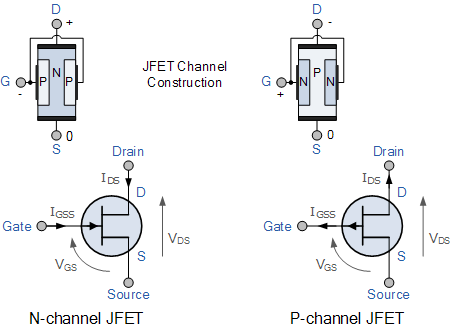
\includegraphics[width=10cm]{src/transistor-tran17.png}
    \caption{N沟道和P沟道场效应管}
\end{figure}
N沟道和P沟道场效应管分别有符号\tikz[baseline=0.0cm] \draw (0,0) node[njfet] {}; 和\tikz[baseline=0.0cm] \draw (0,0) node[pjfet] {};. N沟道的P区高掺杂. 连接后引出\emph{栅极}g, 以及\emph{漏极}d和\emph{源极}s. P区与N区交界面形成耗尽层, 漏极与源极间的非耗尽层谓\emph{导电沟道}.
\par
场效应管的正常工作要求$u\+_GS_ < 0$, $u\+_DS_ > 0$.
\begin{cenum}
    \item 当$u\+_DS_ = 0$, 若$u\+_GS_ = 0$, 则耗尽层窄, 导电沟道宽, 然而$\abs{u\+_GS_}$增加后, 耗尽层变宽, 导电沟道变窄, 到某一$U\+_GS(off)_$后沟道消失, 沟通电阻$\rightarrow \infty$.
    \item 当$u\+_GS_$介于$U\+_GS(off)_$与$0$之间时, 对于非零的$u\+_DS_$, 会有导电通道, 靠近D侧窄, 靠近S侧宽. $u\+_GD_ = u\+_GS_ - u\+_DS_$, 若$u\+_DS_$增加使$u\+_GD_ = U\+_GD(off)_$, 则漏极一侧将出现夹断区. 若$u\+_DS_$继续增加, 则$i_D$近似恒流.
    \item 若$u\+_GD_ = u\+_GS_ - u\+_DS_ <u\+_GS(off)_$, 则可以通过改变$u\+_GS_$以控制$i_D$. 引入低频跨导
    \[ g_m = \left.\frac{\Delta i_D}{\Delta i\+_GS_}\right\vert_{u\+_DS_ = \const}. \]
\end{cenum}
因此有
\begin{cenum}
    \item $u\+_GD_ = u\+_GS_ - u\+_DS_ > U\+_GS(off)_$时, 对于不同$u\+_GS_$, d-s之间等效为不同电阻.
    \item $u\+_GD_ = U\+_GS(off)_$, d-s之间预夹断.
    \item $u\+_GD_ < U\+_GS(off)_$时, $i_D$仅仅取决于$u\+_GS_$, 和$u\+_DS_$无关.
    \item $u\+_GS_ < U\+_GS(off)_$时, $i_D = 0$.
\end{cenum}
\begin{figure}[ht]
    \centering
    \begin{tikzpicture}
        \draw[->] (0,0) node[below left] {$O$} -- (5,0) node[below] {$u\+_DS_$};
        \draw[->] (0,0) -- (0,5) node[left] {$i_D$};
        \draw (0,0) -- (0.1,0.1) -- (4,0.1) node[above left] {$U\+_GS(off)_$} --++(0.2,0.2);
        \draw (0,0) -- (1,1) --(4.1, 1) node[above left] {$\SI{-3}{\volt}$} --++(0.2,0.2);
        \draw (0,0) -- (1.414,2) -- (4.2,2) node[above left] {$\SI{-2}{\volt}$} --++(0.2,0.2);
        \draw (0,0) -- (1.732,3) -- (4.3,3) node[above left] {$\SI{-1}{\volt}$}  --++(0.2,0.2);
        \draw (0,0) -- (2,4) --(4.4,4) node[above left] {$U\+_GS_ = 0$}  --++(0.2,0.2);
        \draw (0,4) node[right] {可变电阻区};
        \draw (2.5,2.5) node {恒流区};
        \draw (3,0.1) -- (2.5,-0.5) node[below] {夹断区};
        \draw (5,3.5) node {击穿区};
        \draw (2,4) -- (2.4,5) node[right] {预夹断轨迹};
        \draw[dashed] plot[smooth] coordinates{(0.0,0.0) (1,1) (1.414,2) (1.732,3) (2,4) (2.32,5)};
        \draw[dashed] plot[smooth] coordinates {(3.99,0) (4.0,0.1) (4.1,1) (4.2,2) (4.3,3) (4.4,4) (4.5,5)};
    \end{tikzpicture}
    \caption{JFET的输出特性}
    \label{fig:JFET输出特性}
\end{figure}
\begin{figure}[ht]
    \centering
    \begin{tikzpicture}
        \draw[->] (-5,0) -- (1,0) node[below] {$u\+_GS_$};
        \draw[->] (0,0) -- (0,4.1) node[left] {$i_D$};
        \draw[domain=-4:0] plot function {4*(1+x/4)*(1+x/4)} node[right] {$I\+_DSS_$};
        \draw (-4,0) node[above left] {$U\+_GS(off)_$};
    \end{tikzpicture}
    \caption{JFET的转移特性}
    \label{fig:JFET转移特性}
\end{figure}
输出特性曲线, 即$u\+_GS_$为常量时, $i_D$与$u\+_DS_$之间的关系, 如\cref{fig:JFET输出特性}. 转移特性曲线, 即$u\+_DS_$为常量时, $i_D$与$u\+_GS_$之间的关系, 如\cref{fig:JFET转移特性}. 实际上,
\[ i_D = I\+_DSS_ \pare{1-\frac{u\+_GS_}{U\+_GS(off)_}}^2,\quad U\+_GS(off)_ < u\+_GS_ < 0. \]
其中$I\+_DSS_$是$u\+_GS_ = 0$发生预夹断时的饱和漏极电流.

% subsubsection 结型场效应管 (end)

\subsubsection{绝缘栅型场效应管} % (fold)
\label{ssub:绝缘栅型场效应管}

绝缘栅型场效应管(IGFET), 通常谓MOS管(MOSFET), 分为N/P沟道增强/耗尽型管.
\begin{figure}[ht]
    \centering
    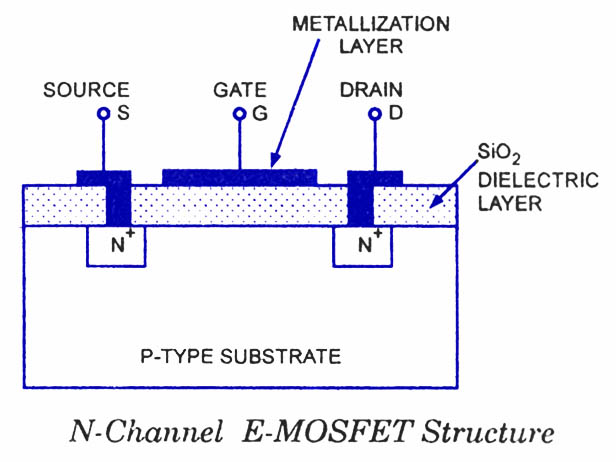
\includegraphics[width=6cm]{src/n-channel-e-mosfet-structure.jpg}
    \caption{N沟道增强型MOS管}
    \label{fig:N沟道增强型MOS管}
\end{figure}

\paragraph{N沟道增强型MOS管} % (fold)
\label{par:n沟道增强型mos管}

\begin{figure}[htb]
    \centering
    \begin{tikzpicture}
        \draw[->] (0,0) node[below left] {$O$} -- (5,0) node[below] {$u\+_DS_$};
        \draw[->] (0,0) -- (0,5) node[left] {$i_D$};
        \draw (0,0) -- (0.1,0.1) -- (4,0.1) node[above right] {$U\+_GS1_=U\+_GS(th)_$} ;
        \draw (0,0) -- (1,1) --(4.1, 1) node[above right] {$U\+_GS1_$} ;
        \draw (0,0) -- (1.414,2) -- (4.2,2) node[above right] {$U\+_GS2_$};
        \draw (0,0) -- (1.732,3) -- (4.3,3) node[above right] {$U\+_GS3_$};
        \draw (0,0) -- (2,4) --(4.4,4) node[above right] {$U\+_GS4_=2U\+_GS(th)_$};
        \draw[dashed] (4.4,4) -- (0,4) node[left] {$I\+_DO_$};
        \draw (0,5) node[right] {可变电阻区};
        \draw (2.5,2.5) node {恒流区};
        \draw (3,0.1) -- (2.5,-0.5) node[below] {夹断区};
        \draw (2,4) -- (2.4,5) node[right] {预夹断轨迹};
        \draw[dashed] plot[smooth] coordinates{(0.0,0.0) (1,1) (1.414,2) (1.732,3) (2,4) (2.32,5)};
    \end{tikzpicture}
    \caption{NEMOSFET的输出特性}
    \label{fig:NEMOSFET输出特性}
\end{figure}
\begin{figure}[htb]
    \centering
    \begin{tikzpicture}
        \draw[->] (0,0) -- (5,0) node[below] {$u\+_GS_$};
        \draw[->] (0,0) -- (0,4.3) node[left] {$i_D$};
        \draw[domain=2:4] plot function {4*(x/2-1)*(x/2-1)} node[right] {$I\+_DO_$};
        \draw (2,0) node[below] {$U\+_GS(th)_$};
        \draw (4,0) node[below] {$2U\+_GS(th)_$};
        \draw[dashed] (4,0) -- (4,4) -- (0,4);
    \end{tikzpicture}
    \caption{NEMOSFET的转移特性}
    \label{fig:NEMOSFET转移特性}
\end{figure}

N沟道增强型MOS管的构造如\cref{fig:N沟道增强型MOS管}, 符号为\tikz[baseline=0.0cm]\draw node[nigfete]{};. N区高掺杂, 中间\ce{SiO_2}为绝缘层. $u\+_GS_$变化时, 改变衬底绝缘层处感应电荷的多少从而控制漏电电流的大小.

\begin{cenum}
    \item $u\+_GS_=0$时, 漏/源之间是两只背向的PN结, 无电流.
    \item 当$u\+_DS_ = 0$, $u\+_GS_ > 0$, 由于绝缘层的存在, 栅极电流为零, 但金属层将聚集正电荷, 排斥P衬底的空穴, 形成耗尽层. $u\+_GS_$增大时, 会在耗尽层与绝缘层之间形成反型层, 可以在漏-源之间形成导电沟道. 此时的栅源电压谓\emph{开启电压}$U\+_GS(th)_$.
    \item 当$u\+_GS_ > U\+_GS(th)_$时, 非零的$u\+_DS_$会产生一定的漏极电流.
    \item 当$u\+_DS_$增加到使得$u\+_GD_ = U\+_GS(th)_$, 出现预夹断, 其后$u\+_DS_$即使增加$i_D$亦维持恒定. 若$u\+_DS_ > u\+_GS_ - U\+_GS(th)_$, 则对应于每一个$u\+_GS_$有一个确定的$i_D$, 从而$u\+_GS_$此时控制$i_D$.
\end{cenum}

对于转移特性, $i_D$和$u\+_CS_$之间有近似关系
\[ i_D = I\+_DO_ \pare{\frac{u\+_GS_}{U\+_GS(th)_}-1}^2. \]

% paragraph n沟道增强型mos管 (end)

\paragraph{N沟道耗尽型MOS管} % (fold)
\label{par:n沟道耗尽型mos管}

N沟道耗尽型MOS管符号为符号为\tikz[baseline=0.0cm]\draw node[nigfetd]{};. \ce{SiO_2}绝缘层中掺入大量正离子, 那么即使$u\+_GS_ = 0$, 在正离子的作用下漏-源之间也存在导电沟道. 此时需要将$u\+_GS_$从零减小至某$u\+_GS(off)_$才能令导电沟道消失, $i_D = 0$.

% paragraph n沟道耗尽型mos管 (end)

\paragraph{P沟道MOS管} % (fold)
\label{par:p沟道mos管}

P沟道增强型MOS管的符号为\tikz[baseline=0.0cm]\draw node[pigfete]{};. 相应的开启电压$U\+_GS(th)_ < 0$, 当$u\+_GS_ < U\+_GS(th)_$时才导通. P沟道耗尽型MOS管的符号为\tikz[baseline=0.0cm]\draw node[pigfetd]{};, 相应的$U\+_GS(off)_ > 0$.

% paragraph p沟道mos管 (end)

\par
如果MOS管的衬底不合源极相连接, 则$U\+_BS_$须保证衬-源间的PN结反向偏置. N沟道管的$U\+_BS_$应小于零, P沟道管反之.

% subsubsection 绝缘栅型场效应管 (end)

\subsubsection{场效应管的主要参数} % (fold)
\label{ssub:场效应管的主要参数}

\begin{cenum}
    \item 开启电压$U\+_GS(th)_$: 适用于增强MOS管, 即$U\+_DS_$为一常量时, 使$i_D$大于零所需最小的$\abs{u\+_GS_}$.
    \item 夹断电压$U\+_GS(off)_$: 适用于结型场效应管和耗尽型MOS管, 即$U\+_DS_$为一常量时, $i_D$逼近零时的$u\+_CS_$.
    \item 饱和漏极电流$I\+_DSS_$: 适用于结型场效应管, 是$u\+_GS_ = 0$时的预夹断漏极电流.
    \item 直流输入电阻$R\+_GS(DC)_$: 等于栅-源电压与栅-极电压之比.
    \item 低频跨导$g_m$: 适用于恒流区内, 和$i_D$具体大小相关,
    \[ g_m = \left.\frac{\Delta i_D}{\Delta u\+_GS_}\right\vert_{U\+_DS_ = \const}. \]
    \item 极间电容$C\+_gs_$, $C\+_gd_$和$C\+_ds_$.
    \item 最大漏极电流$I\+_DM_$: 正常工作时$i_D$的上限.
    \item 击穿电压: 恒流区内使$i_D$骤然增大的$u\+_DS_$.
    \item 最大耗散功率$P\+_DM_$.
\end{cenum}

\begin{sample}
    \begin{ex}
        某管子的输出特性如图, 分析其类型.
    \end{ex}
    \centerline{
    \begin{tikzpicture}
        \draw[->] (0,0) node[below left] {$O$} -- (5,0) node[below] {$u\+_DS_/\SI{}{\volt}$};
        \draw[->] (0,0) -- (0,5) node[left] {$i_D/\SI{}{\milli\ampere}$};
        \draw (0,0) -- (0.1,0.1) -- (3.5,0.1) node[right] {$\SI{4}{\volt}$};
        \draw (0,0) -- (0.5,0.5) -- (3.5,0.5) node[right] {$\SI{6}{\volt}$};
        \draw (0,0) -- (0.707,2) -- (3.5,2) node[right] {$\SI{8}{\volt}$};
        \draw (0,0) -- (1,4) -- (3.5,4) node[right] {$\SI{10}{\volt}$};
        \draw[dashed] (0,0.5) node[left] {$0.25$} -- (0.5,0.5);
        \draw[dashed] (0,2) node[left] {$1$} -- (0.707,2);
        \draw (0,4) node[left] {$2$};
        \draw (0.5,0) node[below] {$3$} (1,0) node[below] {$6$} (1.5,0) node[below] {$9$} (2,0) node[below] {$12$} (2.5,0) node[below] {$15$};
    \end{tikzpicture}
    }
    \begin{solution}
        由曲线图分布在第一象限知其为N类. 由开启电压$U>0$知其为增强型MOS管.
    \end{solution}
\end{sample}

\begin{sample}
    \begin{ex}
        电路如图, 管子的特性曲线和前一题相同. 分析当$u_1$分别为$\SI{0}{\volt}$, $\SI{8}{\volt}$和$\SI{10}{\volt}$时$u_O$分别为多少.
    \end{ex}
    \centerline{
    \begin{tikzpicture}
        \draw (0,0) node[nigfete] (mos) {};
        \draw (mos.G) to[short,-o] ($(mos.G) + (-1,0)$);
        \draw ($(mos.G) + (-1,0)$) node (gout) {};
        \draw (mos.D) to[short,-o] ($(mos.D) + (1.5,0)$);
        \draw ($(mos.S) + (0,-1.5)$) node (sout) {};
        \draw (mos.S) to[short,-*] ($(mos.S) + (0,-1.5)$) node[ground]{} to[short,-o] (gout|-sout);
        \draw ($(mos.S) + (0,-1.5)$) to[short,-o] ($(mos.S) + (1.5,-1.5)$);
        \draw (mos.D) to[resistor,R=$\stackrel{\displaystyle R_d}{\scriptstyle\SI{5}{\kilo\ohm}}$,-o] ($(mos.D) + (0,1.5)$) node[right] {$\stackrel{\displaystyle +V\+_DD_}{\scriptstyle\pare{\SI{+15}{\volt}}}$};
        \draw ($(mos.G) + (-1,0)$) to[open,v=$u_1$] (gout|-sout);
        \draw ($(mos.D) + (1.5,0)$) to[open,v=$u_O$] ($(mos.S) + (1.5,-1.5)$);
    \end{tikzpicture}
    }
    \begin{solution}
        当$u\+_GS_ = u_1 = 0$, 管子处于夹断状态, $i_D = 0$, $u_O = \SI{+15}{\volt}$.
        \par
        当$u\+_GS_ = u_1 = \SI{8}{\volt}$, 令$i_D=\SI{1}{\milli\ampere}$, $u\+_DS_ = \SI{10}{\volt} > u\+_GS_ - U\+_GS(th)_$, 在恒流区内, 故$u_O = \SI{10}{\volt}$.
        \par
        当$u\+_GS_ = u_1 = \SI{10}{\volt}$, 令$i_D=\SI{2.2}{\milli\ampere}$发现$u_O = \SI{4}{\volt}$, 小于夹断电压$u\+_GS_ - U\+_GS(th)_ = \SI{6}{\volt}$. 此时将其等效为电阻,
        \[ R\+_DS_ = \frac{U\+_DS_}{I_D} \approx \pare{\frac{3}{1\times 10^{-3}}}\SI{}{\ohm} = \SI{3}{\kilo\ohm}. \]
        因此相应的
        \[ u_O = \frac{R\+_DS_}{R_d + R\+_DS_} = \SI{5.6}{\volt}. \qedhere \]
    \end{solution}
\end{sample}

\begin{sample}
    \begin{ex}
        电路如图. 场效应管的夹断电压$U\+_GS(off)_ = \SI{-4}{\volt}$, 饱和漏极电流$I\+_DSS_ = \SI{4}{\milli\ampere}$. 为了保证$R_L$上输出恒流, $R_L$的取值范围如何?
    \end{ex}
    \centerline{\begin{tikzpicture}
        \draw (0,0) node[njfet] (njf) {};
        \draw (njf.S) to[short,-o] ++(1,0) node[right] {$u_O$};
        \draw (njf.S) to[vR,R=$R_L$] ++(0,-1.5) node[ground]{};
        \draw (njf.S) --++(-1,0) |- (njf.G);
        \draw (njf.S) node[circ] {};
        \draw (njf.D) to[short,-o] ++(0,0.1) node[right] {$\stackrel{\displaystyle +V\+_DD_}{\scriptstyle \pare{\SI{+12}{\volt}}}$};
    \end{tikzpicture}}
    \begin{solution}
        恒流区要求$u\+_DS_ > u\+_GS_ - U\+_GS(off)_ = \SI{4}{\volt}$, 从而
        \[ R_L < \frac{U\+_DD_ - \SI{4}{\volt}}{I\+_DSS_} = \SI{2}{\kilo\ohm}. \qedhere \]
    \end{solution}
\end{sample}

% subsubsection 场效应管的主要参数 (end)

% section 常用半导体器件 (end)

\end{document}
